\section{Developing and Assessing a Quantitative Evaluation Metric for Kernel Security}
\label{sec.metric}
%\cappos{possible intro sentence / paragraph...}
As mentioned in the previous section, there has been a lack of reliable quantitative
metrics for the development of kernel security systems. Therefore, our first step
was to develop a quantitative metric that could more accurately identify portions of
the OS kernel that had the highest potential to unleash inherent bugs begins with a
hypothesis based on observation and common sense. In this section, we show how we
went about documenting the accuracy of the statement below.

kernel paths that are executed by common applications
during everyday use are less likely to contain security flaws.

This key hypothesis posits that by understanding how and when
a line of code in the kernel is used, we can predict its likelihood to
contain a security flaw.
The intuition is that these code paths are very well-tested
due to their constant use, and thus it is much less likely that security bugs
will occur in these lines of code.
%Since there are relatively few security
%bugs disclosed (dozens) compared to the total number of lines of kernel
%code (millions),

%To test this hypothesis we conducted the following experiment.



%The first step to addressing the threat articulated above is to establish metric
%by which kernel security can be quantitatively evaluated. In this section
%we document the development of such a metric.
%First, we look at current commonly used metrics for code complexity and why they may be less than effective.
%The next section discusses our proposed metric, which focuses on using the kernel code paths accessed by widely used applications.
%Finally, we use the metric to verify our central hypothesis, by testing for the presence of 40 severe Linux  Kernel bugs.

%\lois{This intro section needs work. I'm not happy with what is  here, though I think it is somewhat clearer than what was there before.}

%Before a metric can be developed to meet the threat outlined in Section 2, we need to
%establish a better understanding of basic kernel behavior, and review what we know about
%the risk inherent in privileged code. This section briefly touches on past risk
%metrics, as well as the key hypothesis used to guide the capture and evaluation
%of kernel traces in our study.




%\subsection{Key Hypothesis}
%
%Our metric development begins with the positing of a hypothesis
%that kernel paths executed by popular applications, such as Web browsers or
%text editors, are likely to contain fewer exploitable bugs than uncommonly used paths.
%As they are frequently used, bugs and vulnerabilities in these common kernel
%paths are more likely to have been caught by developers.
%
%In putting forth this hypothesis, we narrow our ``common paths" definition
%to also exclude widely used system calls if they include rare arguments
%and flags. The proposed metric also excludes odd execution paths through popular
%system calls.

\subsection{Experiment Setup}

To test our hypothesis we performed an analysis of two different versions of
the Linux kernel, 3.13.0 and 3.14.1.  Our findings for these
versions are quantitatively and qualitatively similar, so we report
the results for 3.13.0 in this section and use 3.14.1 in Section~\ref{sec.evaluation}.
%\cappos{Fix the version here please.}
To trace the kernel, we used \texttt{gcov}~\cite{gcov}. A standard utility with
the GNU compiler collection (GCC) suite,
\texttt{gcov} is a program profiling tool that indicates which lines of kernel
code are executed while an application runs.

\textbf{Commonly-used kernel paths.}
To capture the commonly-used kernel paths, we used two strategies concurrently.
First, we attempted to capture the normal usage behavior of popular applications.
To do this, two students used
applications in the 50 most popular Debian packages~\cite{Top-Packages}
(omitting libraries) for Debian 7.0.
%Since many such packages are libraries that other programs
%depend on, this resulted in using 50 \cappos{Exactly 50?} \yiwen{Yes. Exactly 50. We chose to stop when we have 50 of them working.} applications.
Each student used 25 applications for their designed
tasks (i.e., writing, spell checking, and then printing a letter in a text
editor, or recoloring and adding a caption to a picture in image processing
software). In instances where there were two applications that performed a
similar task (i.e., Mozilla Firefox and Google Chrome), both programs were
used. These tests were completed over 20 hours of
total use over 5 calendar days.
%\cappos{Were the results the same for the two students?  What percent of LOC varied?}

The second strategy was to try to capture the total range of usages for a
specific computer user. Hence the students used the workstation as their
desktop machine for a one week period. They did their homework, developed
software, communicated with friends and family, etc., using this system.
Software was installed as needed.

Using these two strategies, we obtained a profile of the lines of
kernel code (publicly available at~\cite{Lind}), that indicate
a set of commonly-used kernel paths.

%\cappos{What does the following text actually mean?}
%\yiwen{The following file system operations should belong to the second strategy about
%uses for a specific computer user. The student performed file system operations, like creating
%a folder, deleting a file, etc. during his daily use of the computer, which is part of our test.}
%Several other operations needed to access common paths were conducted, including
%intensive file management tasks to create/read/update or delete files and
%directories from the underlying filesystem.

%The first step in proving our hypothesis was to capture the lines of kernel
%code executed when running applications.
%The OS kernel code
%is organized under different kernel directories.
%Whenever an application tries to access system resources, such as file
%system, I/O and memory, the kernel code under the corresponding paths is executed. Therefore,
%its code execution reflects the basic behavior of the kernel, in response
%to user application requests. To better understand this, we identified and
%captured which lines of code in the kernel
%were executed when running a user program, and named them  \textit{kernel traces}.
%Because these traces are closely related to the program that generates them, it is
%possible to compare different security systems.
%To capture kernel traces, we used \texttt{gcov} \cite{gcov}, a program profiling
%tool that is a standard utility with the GNU compiler collection
%(GCC) suite.

\textbf{Locating bugs.}
Having identified the kernel paths used during application execution, we next
addressed how bugs are distributed in these paths. We collected a list of
severe kernel bugs from the National Vulnerability Database~\cite{NVD}.
%the U.S. government repository of standards-based vulnerability management
%data~\cite{NVD}.
For each bug, we
found the patch that fixed the problem and identified
which lines of kernel code were modified to remove the bug.
For the purpose of this study, a user program that can execute a line of kernel
code changed by such a patch is considered to have the \textit{potential to
exploit that flaw}.  Note, it is possible that in some situations this may
overestimate the ability for an attacker to exploit a flaw, since it may be
possible that additional lines of code must also be executed.


%We determined that any lines of code in the kernel would be considered risky
%if they triggered one or more vulnerability. Other lines of code
%that did not trigger a vulnerability would be considered to be safe to access.
%These lines of code would then compose the common (or safe) portion of the kernel,
%which can be trusted to build a secure trusted computing base for secure systems.
\subsection{Results and Analysis}
\label{Verification-of-Hypothesis}


%To test the hypothesis that commonly used kernel paths contain fewer bugs, we needed
%to identify these paths as a subset of the total reachable kernel paths.
%
%\textbf{Total Reachable Kernel Paths}
%The next step was to obtain the total reachable paths and then analyze the location of
%any vulnerabilities. To accomplish this, we conducted two separate operations.
%
%\begin{enumerate}
%During this step, we conducted

%\textit{System Call Fuzzing}
%System call fuzzing experiments were designed to utilize the Trinity
%system call fuzz tester~\cite{Trinity}. These included sequential execution of
%more than 300 system calls with 1 million iterations
%for executing each system call by 16 child processes (Trinity workers).
%The obtained kernel trace comprehensively reflected various aspects of the
%kernel functionalities.

%\textit{Linux Test Project}
%Linux Test Project (LTP) \cite{LTP} is another tool to generate the kernel traces
%for running all the available system call in different scenarios.
%By using LTP we could validate the kernel traces that
%were generated by Trinity or catch the possible traces that were missing.
%
%\textbf{CVE Bug Reports}
%The last test needed to verify our hypothesis was to check which portions of
%the kernel contained bugs. This was accomplished done by comparing the kernel
%traces with the lines of code we labeled for each bug, based on change of lines in the
%kernel patch. We examined 40 severe Linux kernel
%bugs that had been discovered by the research community in the last five
%years (represented by the first two columns in Table
%\ref{table:vulnerabilities_commonly_used_kernel_paths}).
%The bugs chosen from the NVD bug database have the highest severity score.
%
%\subsubsection{Results and Evaluation}
We now examine our hypothesis given traces for the commonly-used kernel
paths and the set of lines that were patched to fix bugs. We found that
only one of the 40 kernel bugs falls within the commonly-used paths, despite
the commonly-used kernel paths making up 12.4\% of the kernel.
To verify that bugs are more likely to appear in certain parts of
the kernel, we performed the following analysis.

%\cappos{Draft statistical analysis text from Dan.  Needs work...}
We assume that kernel bugs appear at an average rate proportional to the
number of lines of kernel code, and independently of the time since the last
bug occurrence. Therefore, the rate of defect occurrence per LOC
follows a Poisson distribution~\cite{Poisson-distribution}.
%For analysis, we chose to model the rate of defect occurrence per LOC as
%drawn from a Poisson distribution since we believe each bug occurs
%independently, at a constant rate, proportional to the number of lines of
%code, and they do not overlap each other.
This is consistent with the work of Mayer, et. al.~\cite{mayer1989probability}.
%\cappos{Convert the following to a citation: (Mayer, Alan, and Alan Sykes.
%"A probability model for analysing complexity metrics data." Software
%Engineering Journal 4.5 (1989):254-258.)}.
Our hypothesis is that bugs occur at different rates in different parts of the kernel,
i.e., the risky portion has more bugs. Without
loss of generality, we assume that the kernel can be divided into two sections,
$A$ and $B$, where bugs occur at rates $\lambda_A$ and
$\lambda_B$, and $\lambda_A \neq \lambda_B$. Given the null-hypothesis
that the rate of defect occurrences is the \textit{same} in set $A$ and $B$
(or bugs in $A$ and $B$ are drawn from the same Poisson distribution),
%To validate our hypothesis we tested the null-hypothesis that bugs
%occur at the same rate in SET-A and SET-B.
we used the Uniformly Most Powerful Unbiased (UMPU) test~\cite{shiue1982experiment}
%\cappos{Convert this too please: (Shiue,
%Wei-Kei, and Lee J. Bain. "Experiment
%size and power comparisons for two-sample Poisson tests." Applied
%Statistics (1982): 130-134.)}
to compare unequal-sized code blocks.
%We used the R package rateratio.test to perform the calculation.
At a significance level of $\alpha=0.01$, the test was significant at
$\rho=0.0015$, rejecting the null-hypothesis.
%that both sets of bugs are drawn from the same distribution.
The test also reported a 95\% confidence interval that $\lambda_A / \lambda_B
\in [0.002, 0.525]$. This indicates that ratios between bug-rates in each set are well
below 1, and $B$ is the risky set that tends to have more bugs.
%\yanyan{which set is the risky set? e.g., we can say the ratio
%$\lambda_A / \lambda_B<<1$ so that B is the risky set.}\lois{maybe this is just
%echoing Yanyan, but could we get one more sentence that explains in words, not numbers,
%what these numbers mean?}
%\yiwen{We have set A and set B in the kernel. Set A represents the commonly used paths,
%and set B represents the uncommonly used paths. There is 1 bug in set A, and 19 bugs in set B.
%$\lambda_A / \lambda_B<<1$, indicating that B is the risky set that tends to have more bugs.}
In our study, set A represents the commonly used paths in the kernel, while set B represents the uncommonly used paths.
The above statistical results show that set A has a much lower bug rates than set B, which means that the commonly used kernel paths
contain much fewer bugs. Our metric is thus effective in locating bugs in the Linux kernel.

\textbf{Comparison with other metrics.}
Even though there is no widely accepted method for
quantifying the safety (or risk) of privileged code, there have been a number of
attempts to measure flaws in both software and operating systems.
We are not the first to propose a metric for which kernel code may be buggy.
Many metrics work at a coarser granularity (e.g., at file level) than our work that focuses on
individual lines of code.  This is particularly key because at a file
granularity, we found that commonly used programs used parts of
32 files that contained flaws. In fact, common
programs executed 36 functions that later were patched to fix security
flaws, indicating the need to better localize bugs.

Earlier work by Ozment, et al.~\cite{ozment2006milk} demonstrated that code that
had been around longer in the BSD kernel tended to have fewer bugs.
They determined that a significant extent (61\%) of the reported
vulnerabilities were ``foundational," meaning they were introduced prior to the
initial version studied. They also reported these vulnerabilities
have a median lifetime of at least 2.6 years.
We used their metric on our Linux kernel code and our 40 bug dataset.
Based on their metric, we put the Linux kernel code into different age groups.
Our results show that the 40 bugs were not clustered in any particular age group.
Which means that buggy code in the Linux kernel cannot be identified effectively
by simply using their metric.

Chou, et al.~\cite{PittSFIeld} showed that certain parts of the kernel
were more vulnerable than others. In particular, device drivers have
much higher error rates than those in other parts of the kernel.
Applying this metric on our dataset, we found that the driver code in our version
of Linux kernel was only 8.9\% of the total codebase, which contains merely 4 out of 40 bugs.
Using this metric proves to be difficult with the Linux kernel, since our results show that
only 10.0\% of the kernel bugs could be detected.

However, this led us to consider that perhaps since drivers are not used
in many scenarios, code that is unreachable in some situations may have a
different vulnerability profile.  To test this, we
further examined the reachable lines of
code within the kernel using two techniques.  First,
we performed system call fuzzing experiments with the Trinity
system call fuzz tester~\cite{Trinity}. These included 16 child processes
(Trinity workers) executing each Linux system call with 1 million iterations.
Second, we used the Linux Test Project (LTP)~\cite{LTP}, a test suite written
using detailed kernel knowledge.
This test suite is meant to exercise the existing Linux system call interface to
test its correctness, robustness, and performance impact.

The (primarily) black box fuzzing technique from Trinity and test suite of
LTP combine to reach 44.6\% of the kernel, including all 12.4\% of common
paths.  The security in the reachable portion is actually
slightly higher than the unreachable portion.  This is true despite
approximately 1/3 of this code, the commonly-used paths, only containing
a single flaw.  This means that the rate of bug occurrence in reachable, but
not commonly-used kernel paths is actually higher than that in unused
code.  We speculate that this may be because of a higher rate of bug discovery
in code that is available to execute in diverse configurations.


%\textbf{Metric Conclusion}
To summarize, we demonstrated that the metric of looking at commonly-used
kernel paths provides a statistically significant ($\alpha=0.01$,
$\rho=0.0015$) means for predicting where in the kernel exploitable flaws
will be found in the future.  For the remainder of the paper, we will
focus on using this result to build more secure systems.


\begin{figure}%[h]
\centering
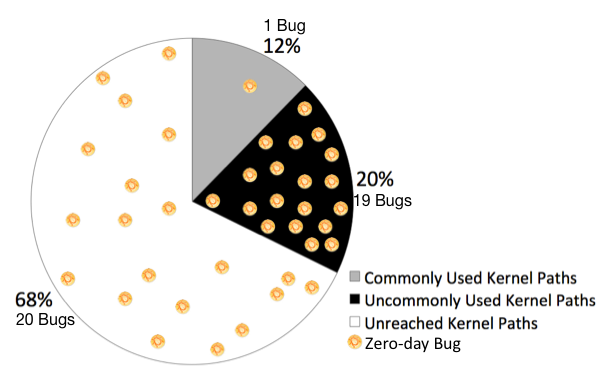
\includegraphics[width=1.0\columnwidth]{diagram/kernel_coverage.png}
\caption{\small Percentage of different kernel areas that were reached during
 LTP and Trinity system call fuzzing experiments, with the zero-day kernel bugs identified
 in each area.}
\label{fig:coverage}
\end{figure}
